\textcolor{blue}{\textbf{Exercício \paragraphnum: 02/09 }
	Considere duas cargas pontuais idênticas separadas por uma distância finita no vácuo. Faça a integral de superfície do tensor dos estresses de Maxwell sobre o plano dos pontos equidistantes às duas cargas. Deduza, assim, a força de Coulomb entre as duas cargas.}
\bigskip\\

Pelo que vimos até o momento a força pode ser escrita considerando o tensor de estresse me Maxwell e o vetor de Poynting a partir das equações de conservação de momento.

\begin{equation}
	\frac{d}{dt}\textbf{P}_m = \textbf{F}_V = \oint da \quad T_{km}n_m - \frac{d}{dt}\int_{V_\infty} d^3r \textbf{S}
\end{equation}

Como no problema atual não dependemos da evolução temporal do sistema podemos desconsiderar os termos dependentes de t, isto é,

\begin{equation}
	\textbf{F}_V = \oint da \quad T_{km}n_m = \oint da \quad \overset{\leftrightarrow}{\textbf{T}} \cdot \hat{\textbf{n}}
	\label{eq3:forca}
\end{equation}

Agora, para calcularmos a integral de superfície sobre o tensor de estresse de Maxwell temos que visualizar um pouco da geometria do problema exemplificado pela figura \ref{fig1:problema}.

\begin{figure}[h]
	\centering
	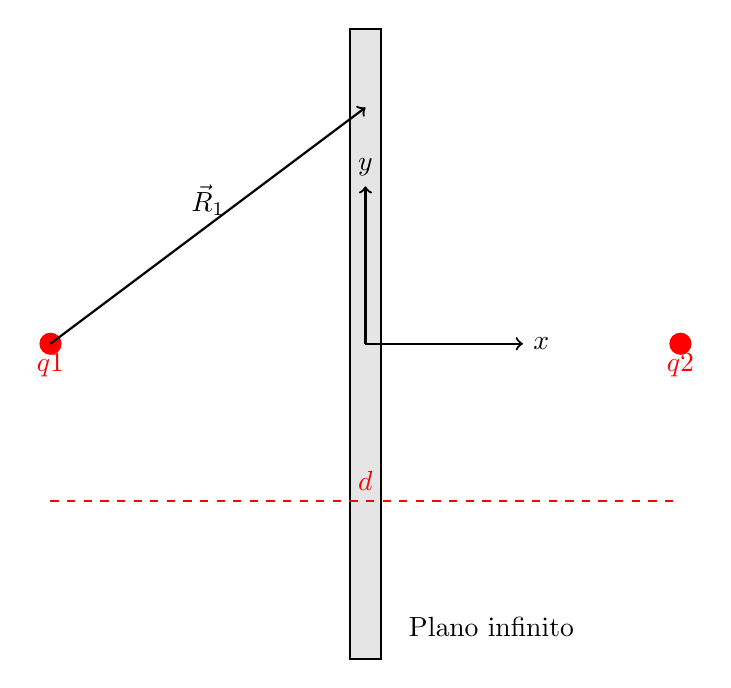
\begin{tikzpicture}[scale=2,thick]
		\centering
		% Definir coordenadas das cargas e plano
		\coordinate (A) at (-2,0);
		\coordinate (B) at (2,0);
		\coordinate (P) at (0,0); % Ponto no plano
		
		% Desenhar o plano perpendicular ao eixo y
		\draw[fill=gray!20] (-0.1,-2) -- (-0.1,2) -- (0.1,2) -- (0.1,-2) -- cycle;
		
		% Desenhar as cargas
		\fill[red] (A) circle (2pt) node[below] {$q1$};
		\fill[red] (B) circle (2pt) node[below] {$q2$};
		
		% Desenhar a linha representando o plano
		%\draw[dashed] (0,-2) -- (0,2);
		
		% Adicionar labels
		\node at (0.8,-1.8) {Plano infinito};
		
		% Adicionar a direção X
		\draw[->] (0,0) -- (1,0) node[right] {$x$};
		
		% Adicionar a direção Y
		\draw[->] (0,0) -- (0,1) node[above] {$y$};
		
		% vetor na até o plano
		\draw[->] (-2,0) -- (0,1.5) node[midway,above] {$\vec{R}_1$};
		
		% Adicionar a direção Y
		\draw[dashed, red] (-2,-1) -- (2,-1) node[midway, above] {$d$};
		
	\end{tikzpicture}
	\caption{Geometria do problema, $\vec{R}$ é o vetor da posição da carga até o plano.}
	\label{fig1:problema}
\end{figure}

Temos que encontrar o campo elétrico total da distribuição de cargas, lembrando que

\begin{equation}
	\textbf{E}_{tot} = \textbf{E}_1 + \textbf{E}_2
\end{equation}

O campo de uma carga pontual no plano será

\begin{equation}
	\textbf{E}_n = \frac{q_n}{R^2} \hat{\textbf{r}_1}
	\label{eq4:campopontual}
\end{equation}
uma vez que $q_n$ é o módulo da n-ésima carga e R a distância entre o ponto do plano e a carga. Portanto o campo elétrico total do sistema pode ser calculado utilizando \ref{eq4:campopontual} para as cargas $q_1$ e $q_2$ com $q_1 = q_2 = q$.

\begin{equation}
	\textbf{E}_{tot} = \frac{q}{ R_1^2}\hat{\textbf{r}}_1+\frac{q}{ R_2^2}\hat{\textbf{r}}_2 = q\left( \dfrac{\hat{\textbf{r}}_1}{R_1^2} + \dfrac{\hat{\textbf{r}}_2}{R_2^2}\right) 
\end{equation}
sendo $\hat{\textbf{r}_n}$ o vetor unitário da direção de $\textbf{R}_n$ e $R_n$ o módulo desse vetor. Podemos escrever esses vetores na forma completa:
\begin{equation}
	\dfrac{\hat{\textbf{r}}_1}{R_1^2} = \frac{\left( \frac{d}{2}\hat{\textbf{x}} + y\hat{\textbf{y}} + z\hat{\textbf{z}}\right)}{\left( \left( \frac{d}{2}\right)^2 + y^2 + z^2 \right)^{\sfrac{3}{2}} } = \frac{\left( \frac{d}{2}\hat{\textbf{x}} + y\hat{\textbf{y}} + z\hat{\textbf{z}}\right)}{\left(\frac{d^2}{4} + y^2 + z^2 \right)^{\sfrac{3}{2}}}
\end{equation}
analogamente,

\begin{equation}
	\dfrac{\hat{\textbf{r}}_2}{R_2^2} = \frac{\left( -\frac{d}{2}\hat{\textbf{x}} + y\hat{\textbf{y}} + z\hat{\textbf{z}}\right)}{\left(\frac{d^2}{4} + y^2 + z^2 \right)^{\sfrac{3}{2}} }
\end{equation}
logo podemos encontrar $\textbf{E}_{tot}$,

\begin{equation}
	\textbf{E}_{tot} = q\left[\frac{\left( \frac{d}{2}\hat{\textbf{x}} + y\hat{\textbf{y}} + z\hat{\textbf{z}}\right)}{\left(\frac{d^2}{4} + y^2 + z^2 \right)^{\sfrac{3}{2}}} +  \frac{\left( -\frac{d}{2}\hat{\textbf{x}} + y\hat{\textbf{y}} + z\hat{\textbf{z}}\right)}{\left(\frac{d^2}{4} + y^2 + z^2 \right)^{\sfrac{3}{2}} }\right] = 2q \frac{y\hat{\textbf{y}} + z\hat{\textbf{z}}}{\left(\frac{d^2}{4} + y^2 + z^2 \right)^{\sfrac{3}{2}} }
\end{equation}

Agora podemos calcular o tensor de estresse de Maxwell diretamente! Lembrando que,

\begin{equation}
	T_{km} = \frac{1}{4\pi}\left(E_k E_m + B_k B_m - \frac{1}{2}\delta_{km}\left(\textbf{E}\cdot\textbf{E}+\textbf{B}\cdot\textbf{B} \right)  \right) 
\end{equation}

logo,

\begin{equation}
	\overset{\leftrightarrow}{\textbf{T}} = \frac{1}{4\pi}
	\begin{pmatrix}
		E_x - \frac{E^2}{2} & E_xE_y & E_xE_z\\
		E_yE_x & E_y - \frac{E^2}{2} & E_yE_z\\
		E_zE_x & E_zE_y & E_z - \frac{E^2}{2}\\
	\end{pmatrix}
	= \frac{1}{4\pi}
	\begin{pmatrix}
		- \frac{E^2}{2} & 0 & 0\\
		0 & E_y - \frac{E^2}{2} & E_yE_z\\
		0 & E_zE_y & E_z - \frac{E^2}{2}\\
	\end{pmatrix}
\end{equation}
uma vez que não temos componentes de campo magnético e as do campo elétrico estão apenas nas direções y e z. Substituindo em \ref{eq3:forca} podemos calcular o valor da força sobre toda a superfície, lembrando que $\hat{\textbf{n}}$ é o versor normal ao plano na direção de x.

\begin{equation}
	\overset{\leftrightarrow}{\textbf{T}}\cdot\hat{\textbf{n}} = \frac{1}{4\pi}
	\begin{pmatrix}
		- \frac{E^2}{2} & 0 & 0\\
		0 & E_y - \frac{E^2}{2} & E_yE_z\\
		0 & E_zE_y & E_z - \frac{E^2}{2}\\
	\end{pmatrix} \cdot
	\begin{pmatrix}
		-1\\0\\0
	\end{pmatrix} =
	\frac{E^2}{2} \hat{\textbf{x}} = \frac{1}{8\pi}4q^2 \frac{y^2 + z^2}{\left(\frac{d^2}{4} + y^2 + z^2 \right)^{3} }\hat{\textbf{x}}
\end{equation}

Lembrando que,

\begin{equation}
	E^2 = \textbf{E}_{tot}\cdot \textbf{E}_{tot} = q^2\frac{y^2+z^2}{\left(\frac{d^2}{4} + y^2 + z^2 \right)^{3}}
\end{equation}
e substituindo esse resultado na integral temos,

\begin{equation}
	\begin{split}
	\textbf{F}_V & = \oint da \quad \overset{\leftrightarrow}{\textbf{T}} \cdot \hat{\textbf{n}} = \oint da \quad \frac{q^2}{2\pi} \frac{y^2 + z^2}{\left(\frac{d^2}{4} + y^2 + z^2 \right)^{3} }\hat{\textbf{x}}\\
	& = \frac{q^2}{2\pi} \int_{-\infty}^{+\infty} dz \int_{-\infty}^{+\infty} dy \frac{y^2 + z^2}{\left(\frac{d^2}{4} + y^2 + z^2 \right)^{3}}\hat{\textbf{x}}\\
	& = \frac{q^2}{2\pi} \int_{0}^{2\pi} d\phi \int_{0}^{+\infty} ds \text{ }s \frac{s^2}{\left(\frac{d^2}{4} + s^2\right)^{3}}\hat{\textbf{x}}\\
	& = \frac{q^2}{2\pi} \int_{0}^{2\pi} d\phi \int_{0}^{+\infty} ds \text{ } \frac{s^3}{\left(\frac{d^2}{4} + s^2\right)^{3}}\hat{\textbf{x}}\\
	\end{split}
\end{equation}

Resolvendo com a substituição de $u = s^2$ e $du = 2sds$ temos,

\begin{equation}
	\int_0^{+\infty}\frac{us}{\left(\frac{d^2}{4} + u\right)^{3}}\frac{du}{2s} = \int_0^{+\infty}\frac{u}{\left(\frac{d^2}{4} + u\right)^{3}}\frac{du}{2} = \frac{1}{d^2}
\end{equation}
além de não termos varíaveis em $\phi$, logo temos a contruibuição $2\pi$ mediante integração. Finalmente temos a força $F_V$ na direção:

\begin{equation}
	\textbf{F}_V = \frac{q^2}{2\pi} \frac{2\pi}{d^2} \hat{\textbf{x}}= \frac{q^2}{d^2}\hat{\textbf{x}}
\end{equation}

%%%%%%%%%%%%%%
%\textcolor{blue}{\textbf{Exercício \paragraphnum: 02/09 }
%	Considere duas cargas pontuais idênticas separadas por uma distância finita no vácuo. Faça a integral de superfície do tensor dos estresses de Maxwell sobre o plano dos pontos equidistantes às duas cargas. Deduza, assim, a força de Coulomb entre as duas cargas.}
%\bigskip\\
%
%Pelo que vimos até o momento a força pode ser escrita considerando o tensor de estresse me Maxwell e o vetor de Poynting a partir das equações de conservação de momento.
%
%\begin{equation}
%	\frac{d}{dt}\textbf{P}_m = \textbf{F}_V = \oint da \quad T_{km}n_m - \frac{d}{dt}\int_{V_\infty} d^3r \textbf{S}
%\end{equation}
%
%Como no problema atual não dependemos da evolução temporal do sistema podemos desconsiderar os termos dependentes de t, isto é,
%
%\begin{equation}
%	\textbf{F}_V = \oint da \quad T_{km}n_m = \oint da \quad \overset{\leftrightarrow}{\textbf{T}} \cdot \hat{\textbf{n}}
%	\label{eq3:forca}
%\end{equation}
%
%Agora, para calcularmos a integral de superfície sobre o tensor de estresse de Maxwell temos que visualizar um pouco da geometria do problema exemplificado pela figura \ref{fig1:problema}.
%
%\begin{figure}[h]
%	\centering
%	\begin{tikzpicture}[scale=2,thick]
%		\centering
%		% Definir coordenadas das cargas e plano
%		\coordinate (A) at (-2,0);
%		\coordinate (B) at (2,0);
%		\coordinate (P) at (0,0); % Ponto no plano
%		
%		% Desenhar o plano perpendicular ao eixo y
%		\draw[fill=gray!20] (-0.1,-2) -- (-0.1,2) -- (0.1,2) -- (0.1,-2) -- cycle;
%		
%		% Desenhar as cargas
%		\fill[red] (A) circle (2pt) node[below] {$q1$};
%		\fill[red] (B) circle (2pt) node[below] {$q2$};
%		
%		% Desenhar a linha representando o plano
%		%\draw[dashed] (0,-2) -- (0,2);
%		
%		% Adicionar labels
%		\node at (0.8,-1.8) {Plano infinito};
%		
%		% Adicionar a direção X
%		\draw[->] (0,0) -- (1,0) node[right] {$x$};
%		
%		% Adicionar a direção Y
%		\draw[->] (0,0) -- (0,1) node[above] {$y$};
%		
%		% vetor na até o plano
%		\draw[->] (-2,0) -- (0,1.5) node[midway,above] {$\vec{R}_1$};
%		
%		% Adicionar a direção Y
%		\draw[dashed, red] (-2,-1) -- (2,-1) node[midway, above] {$d$};
%		
%	\end{tikzpicture}
%	\caption{Geometria do problema, $\vec{R}$ é o vetor da posição da carga até o plano.}
%	\label{fig1:problema}
%\end{figure}
%
%Temos que encontrar o campo elétrico total da distribuição de cargas, lembrando que
%
%\begin{equation}
%	\textbf{E}_{tot} = \textbf{E}_1 + \textbf{E}_2
%\end{equation}
%
%O campo de uma carga pontual no plano será
%
%\begin{equation}
%	\textbf{E}_n = \frac{q_n}{4\pi\epsilon_0 R^2} \hat{\textbf{r}_1}
%	\label{eq4:campopontual}
%\end{equation}
%
%uma vez que $q_n$ é o módulo da n-ésima carga e R a distância entre o ponto do plano e a carga. Portanto o campo elétrico total do sistema pode ser calculado utilizando \ref{eq4:campopontual} para as cargas $q_1$ e $q_2$ com $q_1 = q_2 = q$.
%
%\begin{equation}
%	\textbf{E}_{tot} = \frac{q}{4\pi\epsilon_0 R_1^2}\hat{\textbf{r}}_1+\frac{q}{4\pi\epsilon_0 R_2^2}\hat{\textbf{r}}_2 = \frac{q}{4\pi\epsilon_0}\left( \dfrac{\hat{\textbf{r}}_1}{R_1^2} + \dfrac{\hat{\textbf{r}}_2}{R_2^2}\right) 
%\end{equation}
%
%sendo $\hat{\textbf{r}_n}$ o vetor unitário da direção de $\textbf{R}_n$ e $R_n$ o módulo desse vetor. Podemos escrever esses vetores na forma completa:
%\begin{equation}
%	\dfrac{\hat{\textbf{r}}_1}{R_1^2} = \frac{\left( \frac{d}{2}\hat{\textbf{x}} + y\hat{\textbf{y}} + z\hat{\textbf{z}}\right)}{\left( \left( \frac{d}{2}\right)^2 + y^2 + z^2 \right)^{\sfrac{3}{2}} } = \frac{\left( \frac{d}{2}\hat{\textbf{x}} + y\hat{\textbf{y}} + z\hat{\textbf{z}}\right)}{\left(\frac{d^2}{4} + y^2 + z^2 \right)^{\sfrac{3}{2}}}
%\end{equation}
%
%analogamente,
%
%\begin{equation}
%	\dfrac{\hat{\textbf{r}}_2}{R_2^2} = \frac{\left( -\frac{d}{2}\hat{\textbf{x}} + y\hat{\textbf{y}} + z\hat{\textbf{z}}\right)}{\left(\frac{d^2}{4} + y^2 + z^2 \right)^{\sfrac{3}{2}} }
%\end{equation}
%
%logo podemos encontrar $\textbf{E}_{tot}$,
%
%\begin{equation}
%	\textbf{E}_{tot} = \frac{q}{4\pi\epsilon_0}\left[\frac{\left( \frac{d}{2}\hat{\textbf{x}} + y\hat{\textbf{y}} + z\hat{\textbf{z}}\right)}{\left(\frac{d^2}{4} + y^2 + z^2 \right)^{\sfrac{3}{2}}} +  \frac{\left( -\frac{d}{2}\hat{\textbf{x}} + y\hat{\textbf{y}} + z\hat{\textbf{z}}\right)}{\left(\frac{d^2}{4} + y^2 + z^2 \right)^{\sfrac{3}{2}} }\right] = \frac{q}{2\pi\epsilon_0} \frac{y\hat{\textbf{y}} + z\hat{\textbf{z}}}{\left(\frac{d^2}{4} + y^2 + z^2 \right)^{\sfrac{3}{2}} }
%\end{equation}
%
%Agora podemos calcular o tensor de estresse de Maxwell diretamente! Lembrando que,
%
%\begin{equation}
%	T_{km} = \frac{1}{4\pi}\left(E_k E_m + B_k B_m - \frac{1}{2}\delta_{km}\left(\textbf{E}\cdot\textbf{E}+\textbf{B}\cdot\textbf{B} \right)  \right) 
%\end{equation}
%
%logo,
%
%\begin{equation}
%	\overset{\leftrightarrow}{\textbf{T}} = \frac{1}{4\pi}
%	\begin{pmatrix}
%		E_x - \frac{E^2}{2} & E_xE_y & E_xE_z\\
%		E_yE_x & E_y - \frac{E^2}{2} & E_yE_z\\
%		E_zE_x & E_zE_y & E_z - \frac{E^2}{2}\\
%	\end{pmatrix}
%	= \frac{1}{4\pi}
%	\begin{pmatrix}
%		- \frac{E^2}{2} & 0 & 0\\
%		0 & E_y - \frac{E^2}{2} & E_yE_z\\
%		0 & E_zE_y & E_z - \frac{E^2}{2}\\
%	\end{pmatrix}
%\end{equation}
%
%uma vez que não temos componentes de campo magnético e as do campo elétrico estão apenas nas direções y e z. Substituindo em \ref{eq3:forca} podemos calcular o valor da força sobre toda a superfície, lembrando que $\hat{\textbf{n}}$ é o versor normal ao plano na direção de x.
%
%\begin{equation}
%	\overset{\leftrightarrow}{\textbf{T}}\cdot\hat{\textbf{n}} = \frac{1}{4\pi}
%	\begin{pmatrix}
%		- \frac{E^2}{2} & 0 & 0\\
%		0 & E_y - \frac{E^2}{2} & E_yE_z\\
%		0 & E_zE_y & E_z - \frac{E^2}{2}\\
%	\end{pmatrix} \cdot
%	\begin{pmatrix}
%		-1\\0\\0
%	\end{pmatrix} =
%	\frac{E^2}{2} \hat{\textbf{x}} = \frac{1}{8\pi}\frac{q^2}{\left( 2\pi\epsilon_0\right)^2} \frac{y^2 + z^2}{\left(\frac{d^2}{4} + y^2 + z^2 \right)^{3} }\hat{\textbf{x}}
%\end{equation}
%
%Lembrando que,
%
%\begin{equation}
%	E^2 = \textbf{E}_{tot}\cdot \textbf{E}_{tot} = \frac{q^2}{\left( 2\pi\epsilon_0\right)^2}\frac{y^2+z^2}{\left(\frac{d^2}{4} + y^2 + z^2 \right)^{3}}
%\end{equation}
%
%Substituindo esse resultado na integral temos,
%
%\begin{equation}
%	\begin{split}
%		\textbf{F}_V & = \oint da \quad \overset{\leftrightarrow}{\textbf{T}} \cdot \hat{\textbf{n}} = \oint da \quad \frac{1}{8\pi}\frac{q^2}{\left( 2\pi\epsilon_0\right)^2} \frac{y^2 + z^2}{\left(\frac{d^2}{4} + y^2 + z^2 \right)^{3} }\hat{\textbf{x}}\\
%		& = \frac{1}{8\pi}\frac{q^2}{\left( 2\pi\epsilon_0\right)^2} \int_{-\infty}^{+\infty} dz \int_{-\infty}^{+\infty} dy \frac{y^2 + z^2}{\left(\frac{d^2}{4} + y^2 + z^2 \right)^{3}}\hat{\textbf{x}}\\
%		& = \frac{1}{8\pi}\frac{q^2}{\left( 2\pi\epsilon_0\right)^2} \int_{0}^{2\pi} d\phi \int_{0}^{+\infty} ds \text{ }s \frac{s^2}{\left(\frac{d^2}{4} + s^2\right)^{3}}\hat{\textbf{x}}\\
%		& = \frac{1}{8\pi}\frac{q^2}{\left( 2\pi\epsilon_0\right)^2} \int_{0}^{2\pi} d\phi \int_{0}^{+\infty} ds \text{ } \frac{s^3}{\left(\frac{d^2}{4} + s^2\right)^{3}}\hat{\textbf{x}}\\
%	\end{split}
%\end{equation}
%
%Resolvendo com a substituição de $u = s^2$ e $du = 2sds$ temos,
%
%\begin{equation}
%	\int_0^{+\infty}\frac{us}{\left(\frac{d^2}{4} + u\right)^{3}}\frac{du}{2s} = \int_0^{+\infty}\frac{u}{\left(\frac{d^2}{4} + u\right)^{3}}\frac{du}{2} = \frac{1}{d^2}
%\end{equation}
%
%
%além de não termos varíaveis em $\phi$, logo temos a contruibuição $2\pi$ mediante integração. Finalmente temos a força $F_V$ na direção:
%
%\begin{equation}
%	\textbf{F}_V = \frac{1}{8\pi}\frac{q^2}{\left( 2\pi\epsilon_0\right)^2} \frac{2\pi}{d^2} \hat{\textbf{x}}= \frac{q^2}{\left( 4\pi\right)^2} \frac{1}{d^2}\hat{\textbf{x}}
%\end{equation}
%
%Lembrando que estamos trabalhando no CGS, por isso podemos considerar $\epsilon_0 = 1$.
